% \section{Risk analysis} 
% In this section the different threats identified in \cref{sec:threat_model} will be evaluated. The different threats will be listed with their estimated impact and likelihood. The impact describes how the threat are affecting the election and how impactful it would be on a scale from very low to critical. The likelihood describes how likely the threat is to occur on a scale from very low to very high. Additionally control recommendations will be listed to assess how the given likelihood can be lowered or even nullify the threat.

%\subsection{Pre-election phase analysis}
%\subsubsection{Malicious election administrator}
%subsubsection{Opening ceremony}
%\subsubsection{OPT provider}

%\begin{figure}[H]
%    \centering
%    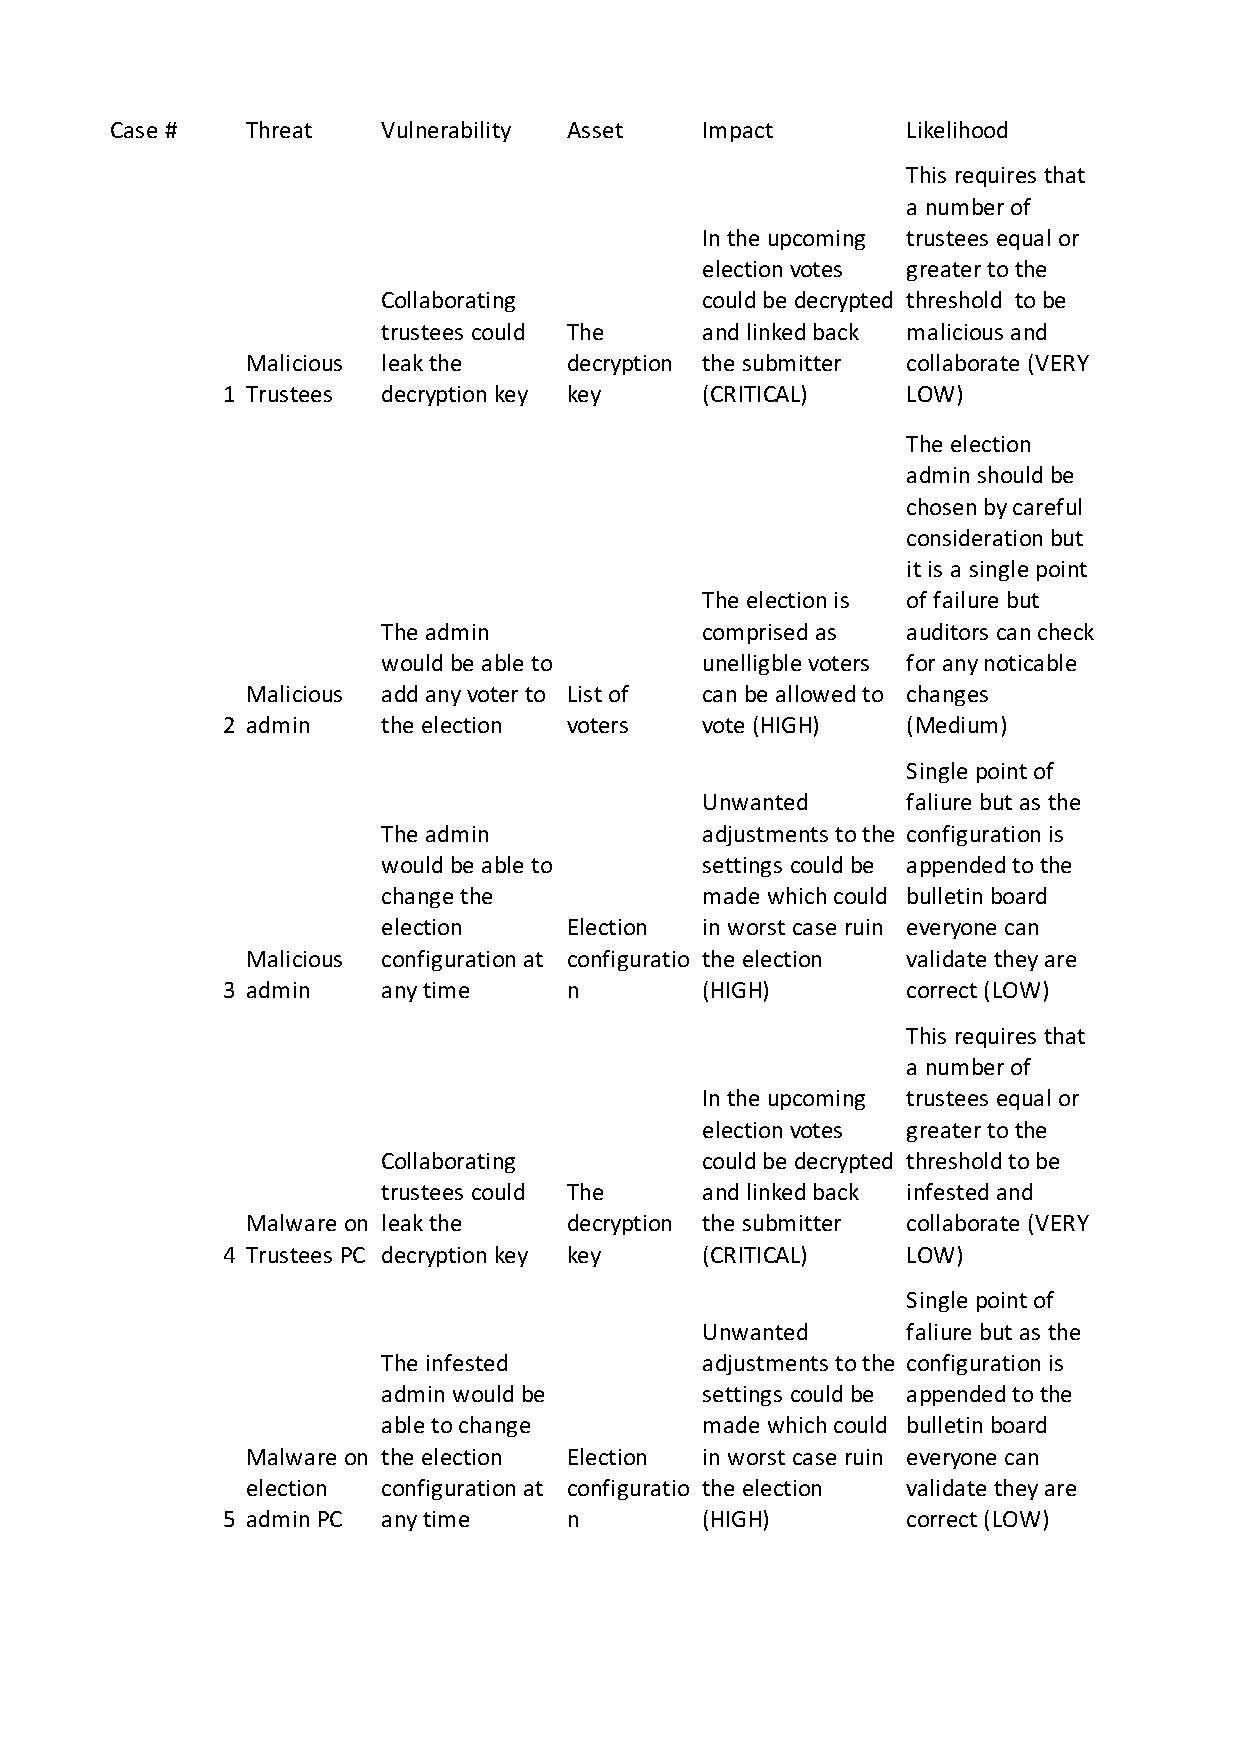
\includegraphics[width=1\textwidth]{Pictures/ThreatRiskAnalysis.pdf}
%    \caption{} e 
%\end{figure}
